\section{Views}
In this section, we present three prototypical views built upon the
presented visualization infrastructure. Therefore, The interaction of the views
provide a scalable top-down approach for identifying hotspots, developing
parallelization strategies, and validating these strategies w.r.t.~data
dependencies.

\subsection{Performance View}
\label{sec:performance_view}
The performance view is an interactive representation of a program's profiling
and trace data. Its primary purpose is to assist users in identifying scenarios
that may benefit from parallelization. A holistic visualization of a program's
runtime behavior helps users to spot potential performance and to guide
optimization efforts.

There are two visualization modes in the performance view: tracing and
profiling. The tracing mode represents an icicle plot augmented with loop
information, i.e., a hierarchical view of calls made during program execution.
The calls are arranged chronologically from left to right, and the visibility
of loop information can be toggled (on or off). Trace visualization is useful
for detailed examination of a program, especially when the traced invocation
order is important. The profiling mode presents the user a hierarchical view of
the functions called during execution. The length of each function in the view
is given by the sum of the calls' duration which is often sufficient to quickly
pinpoint hot spots.

With growing size and complexity of a program, the performance data also
increases, making it harder to digest it at once. For this reason, the
performance view provides zooming at call level and runtime duration filtering.
The latter sets the minimum runtime duration required for a call to be loaded.
The minimum value depends on the percentage of the runtime duration of the
current top-level call in the view. This allows to only render calls large
enough to be easily visible. With the call zooming feature, users can focus on
a specific call, which makes it the top-level call, recomputes a new minimum
value, and loads child calls of the focused call that weren't visible before.

\begin{figure*}[ht!]
	\begin{center}
		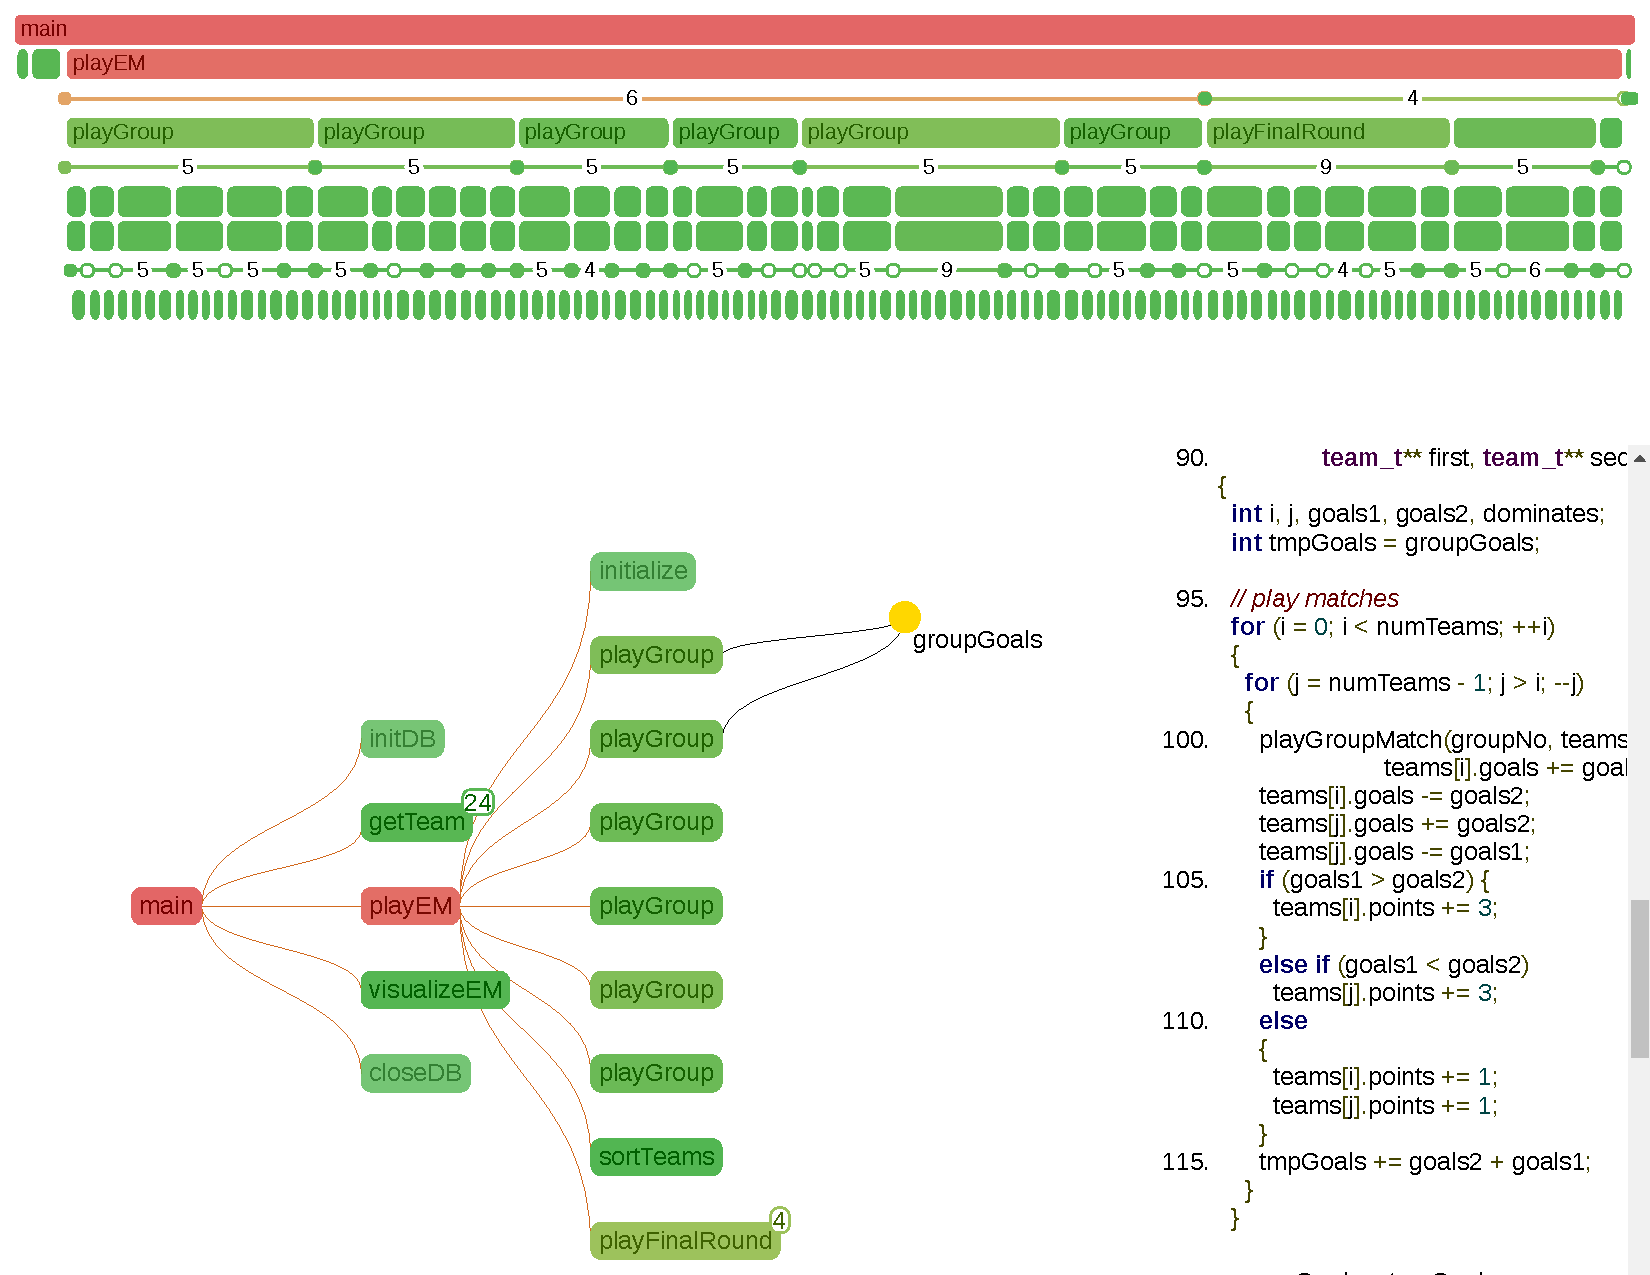
\includegraphics[clip, trim=0.1cm 16.0cm 0.1cm 0.1cm,
width=\linewidth]{img/performance_view.pdf}
		\caption{The performance view of Parceive showing an EMSim trace.}
		\label{fig:emsim}
	\end{center}
\end{figure*}

\subsection{Calling Context Tree (CCT) View}
The CCT view targets comprehension of the dynamic behavior of an application.
It displays a call tree consisting of call nodes, loop nodes, and memory nodes
(see Figure \ref{fig:cct_view}). Nodes for calls (or groups of calls), loop
executions, and loop iterations are positioned using a tidy tree
layout~\cite{TidierTree}. Children of nodes are vertically sorted by their
start time to reflect their actual execution. Memory nodes accessed by
arbitrary tree nodes are difficult to integrate in a tree layout. Therefore,
they are positioned using an unconstrained layout based on a force simulation
around the rest of the tree.

The first node present when the view is created is the call to the
\texttt{main} function. Users can arbitrarily expand and collapse call nodes.
When a function was called multiple times during the same function execution,
the respective call nodes are merged to so-called \textit{call groups}. Call
groups reduce the number of nodes to be displayed but can also be decomposed
into their single call nodes. Navigating through loop executions and loop
iterations is similar to calls and allows the user to see information at any
desired granularity. 

The most important feature of the CCT view for parallelization is data
dependency analysis. Users are often interested in the existence and the
location of such dependencies between arbitrary regions of their software.
Therefore, an optimized query of the visualization infrastructure is utilized
to detect shared memory accesses across deep call hierarchies. Found
dependencies can then be inspected in a separate source code view. The
described feature allows manageable visualization by dramatically reducing the
amount of shown nodes. There are some additional features that aim for better
scalability and help developers parallelizing their code:

\begin{itemize}
	\item Profiling information (relative execution time) is reflected by node
colors.
	\item Expanding and collapsing nodes can be performed in both
directions to show and hide parent or child nodes.
	\item Seamless zooming or panning, and focusing on single entity nodes for
a clear visualization.
	\item Spotting of arbitrary call nodes that automatically expands the call
tree up to these nodes and start with their common ancestor.
\end{itemize}

\begin{figure}[h!]
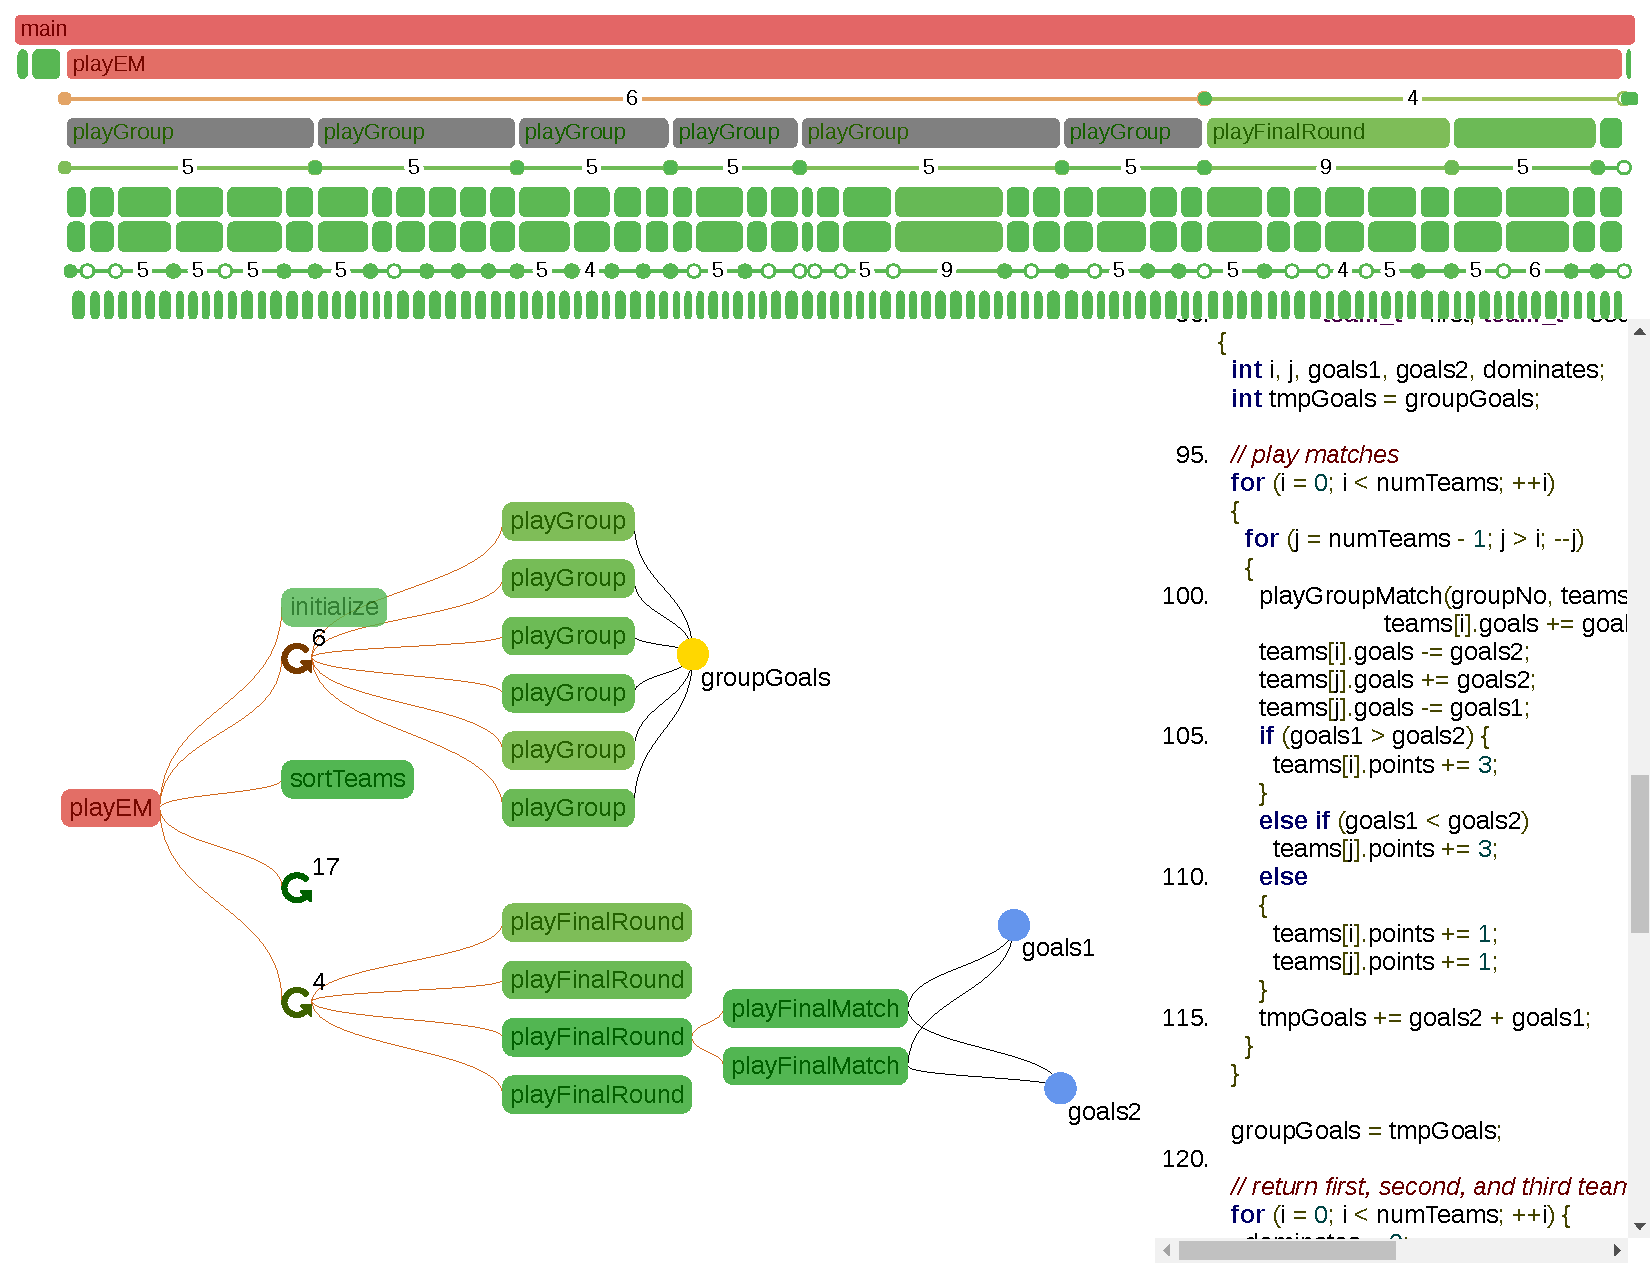
\includegraphics[clip, trim=0.9cm 2.5cm 8.5cm 8.5cm,
width=\linewidth]{img/cct_view}
\caption{The calling context tree view of Parceive.}
\label{fig:cct_view}	
\end{figure}


\subsection{Source View}
The source view shows the highlighted source code that was used to
build the instrumented application. The usefulness of this view becomes
apparent when it is communicating with the other views presented in this paper.
The simplest form of interaction is focusing, where the source view display the
definition of functions, loops, and memory accesses, which makes it easy to
follow the execution of a program trough the source code. Hovering provides
additional information---for calls it indicates where the call originated, and
for memory references where they were allocated and referenced.